% !TEX root = ../thesis.tex

\chapter{\name{Eliashberg} theory}

Based on the results presented in the previous chapter, one can formulate a set
of equations, namely the \name{Eliashberg} equations, which determine
self-energies for both normal and anomalous \name{Green} functions, the latter
being suitable order parameters for the superconducting state.

To that end it is convenient to combine the \name{Green} functions of interest
into a $2 \times 2$ matrix, i.e. to use the \name{Nambu} formalism, which is
presented in the first section. With that, the general form of the
\name{Eliashberg} equations on the imaginary frequency axis is derived, followed
by two common approximations which assume (1) a local self-energy and (2) a
constant density of states. Next, it is shown how the corresponding real-axis
equations can be obtained through analytical continuation. On this basis
\name{McMillan}'s formula for the critical temperature is derived, whereby the
\name{Coulomb} pseudo-potential is introduced. This requires a more detailed
discussion of rescaling of the \name{Coulomb} interaction, leading to results
which are also useful in dealing with the chemical potential. After that, the
whole formalism is generalized to multiple electronic bands. The penultimate
section is dedicated to the determination of the critical temperature via
linearized \name{Eliashberg} equations. Finally, it is demonstrated how
imaginary-axis results can be continued to the real axis by means of \name{Padé}
approximants.

\section{\name{Nambu} formalism}

As found by \name{Nambu} \cite{Nambu60}, the \text{Dyson} equations for all four
electronic \name{Green} functions introduced at the beginning of
Section~\ref{Model interactions} can be compactly formulated as a single matrix
equation. Diagrammatically, within the GW approximation and without
\name{Hartree} contributions, it reads
%
\begin{equation*}
    % !TEX root = ../thesis.tex
%
\tikzsetnextfilename{nambu-dyson}
%
\begin{tikzpicture}[yscale=-1]
    \foreach \r in {
        (-0.25, 0.25), (2.25, 0.25), (4.75, 0.25), (7.00, 0.25), (9.25, 0.25),
        ( 2.25, 1.50), (2.25, 2.75)}
        \node at \r {$\Bigg[$};

    \foreach \r in {
        ( 1.75, 0.25), (4.25, 0.25), (6.75, 0.25), (9.00, 0.25), (11.25, 0.25),
        (12.25, 1.50), (8.25, 2.75)}
        \node at \r {$\Bigg]$};

    \foreach \r in {
        (2.5, 0.00), (5.0, 0.00), ( 2.5, 1.25), (3.5, 1.25),
        (5.5, 1.25), (8.5, 1.25), (10.5, 1.25), (2.5, 2.50),
        (3.5, 2.50), (4.5, 2.50), ( 6.5, 2.50), (4.5, 3.00)}
        \draw [backward] \r -- +(0.5, 0);

    \foreach \r in {(3.75, 0), (6.25, 0), (2.75, 0.5), (5.25, 0.5)}
        \node at \r {$0$};

    \foreach \r in {
        (3.5, 0.50), (6.0, 0.50), ( 3.5, 1.75), (5.5, 1.75),
        (7.5, 1.75), (8.5, 1.75), (10.5, 1.75), (7.5, 2.50),
        (3.5, 3.00), (5.5, 3.00), ( 6.5, 3.00), (7.5, 3.00)}
        \draw [forward] \r -- +(0.5, 0);

    \draw [backward] (4, 2.5) arc (180:360:2.5mm);
    \draw [ outward] (7, 2.5) arc (180:360:2.5mm);
    \draw [  inward] (4, 3.0) arc (180:360:2.5mm);
    \draw [ forward] (7, 3.0) arc (180:360:2.5mm);

    \foreach \r in {(4, 2.5), (7, 2.5), (4, 3), (7, 3)}
        \draw [phonon] \r -- +(0.5, 0);

    \foreach \r in {(0, 0.0), ( 9.5, 0.0), ( 4.5, 1.25), ( 4.5, 1.75)}
        \draw [backward, double] \r -- +(0.5, 0);
    \foreach \r in {(1, 0.0), (10.5, 0.0), ( 9.5, 1.25), ( 9.5, 1.75)}
        \draw [ outward, double] \r -- +(0.5, 0);
    \foreach \r in {(0, 0.5), ( 9.5, 0.5), ( 6.5, 1.25), ( 6.5, 1.75)}
        \draw [  inward, double] \r -- +(0.5, 0);
    \foreach \r in {(1, 0.5), (10.5, 0.5), (11.5, 1.25), (11.5, 1.75)}
        \draw [ forward, double] \r -- +(0.5, 0);

    \foreach \r in {(7.25, 0.0), (4, 1.25), ( 9, 1.25)}
        \draw [backward, double] \r arc (180:360:2.5mm);
    \foreach \r in {(8.25, 0.0), (6, 1.25), (11, 1.25)}
        \draw [ outward, double] \r arc (180:360:2.5mm);
    \foreach \r in {(7.25, 0.5), (4, 1.75), ( 9, 1.75)}
        \draw [  inward, double] \r arc (180:360:2.5mm);
    \foreach \r in {(8.25, 0.5), (6, 1.75), (11, 1.75)}
        \draw [ forward, double] \r arc (180:360:2.5mm);

    \foreach \r in {
        (7.25, 0), (8.25, 0), (7.25, 0.5), (8.25, 0.5),
        (4, 1.25), (6, 1.25), (9, 1.25), (11, 1.25),
        (4, 1.75), (6, 1.75), (9, 1.75), (11, 1.75)}
        \draw [phonon, double] \r -- +(0.5, 0);

    \foreach \r in {
        (7.25, 0), (8.25, 0), (7.25, 0.5), (8.25, 0.5),
        (4, 1.25), (6, 1.25), (9, 1.25), (11, 1.25),
        (4, 1.75), (6, 1.75), (9, 1.75), (11, 1.75),
        (4, 2.50), (7, 2.50), (4, 3.00), ( 7, 3.00)}
        \fill \r circle (1.5pt) +(0.5, 0) circle (1.5pt);

    \foreach \r in {(2, 0.25), (2, 1.5)} \node at \r {$=$};

    \node at (2, 2.75) {$\approx$};

    \foreach \r in {
        (4.50, 0.25),
        (3.25, 1.25), (5.25, 1.25), (8.25, 1.75), (10.25, 1.25),
        (3.25, 2.50), (5.25, 1.75), (6.25, 3.00), (10.25, 1.75)}
        \node at \r {$+$};
\end{tikzpicture}%

\end{equation*}
%
and formally, where quantum numbers and frequency arguments are suppressed,
%
\begin{equation} \label{Nambu-Dyson equation}
    \begin{split}
        \begin{bmatrix}
            G & F \\
            \widetilde F & \widetilde G
        \end{bmatrix}
        &=
        \begin{bmatrix}
            G_0 & 0 \\
            0 & \widetilde G_0
        \end{bmatrix}
        +
        \begin{bmatrix}
            G_0 & 0 \\
            0 & \widetilde G_0
        \end{bmatrix}
        \begin{bmatrix}
            \Sigma^G & \Sigma^F \\
            \Sigma^{\widetilde F} & \Sigma^{\widetilde G}
        \end{bmatrix}
        \begin{bmatrix}
            G & F \\
            \widetilde F & \widetilde G
        \end{bmatrix}
        \\
        &=
        \begin{bmatrix*}[r]
            G_0 + G_0 \Sigma^G G + G_0 \Sigma^F \widetilde F
            & G_0 \Sigma^G F + G_0 \Sigma^F \widetilde G \\
            \widetilde G_0 \Sigma^{\widetilde F} G
            + \widetilde G_0 \Sigma^{\widetilde G} \widetilde F
            & \widetilde G_0 + \widetilde G_0 \Sigma^{\widetilde F} F
            + \widetilde G_0 \Sigma^{\widetilde G} \widetilde G
        \end{bmatrix*}
        \\
        &\approx
        \begin{bmatrix*}[r]
            G_0 + G_0 \Sigma^G_0 G_0 & G_0 \Sigma^F_0 \widetilde G_0 \\
            \widetilde G_0 \Sigma^{\widetilde F}_0 G_0 & \widetilde G_0
            + \widetilde G_0 \Sigma^{\widetilde G}_0 \widetilde G_0
        \end{bmatrix*}.
    \end{split}
\end{equation}

\tikz [baseline=-0.5ex] \draw [ inward] (0, 0) -- (0.8, 0); and
\tikz [baseline=-0.5ex] \draw [outward] (0, 0) -- (0.8, 0);
%
vanish, so does each term of the perturbation series of
%
\tikz [baseline=-0.5ex] \draw [ inward, double] (0, 0) -- (0.8, 0); and
\tikz [baseline=-0.5ex] \draw [outward, double] (0, 0) -- (0.8, 0);.
%
However, a non-zero self-consistent solution of the above integral equations may
also exist \cite[before Eq.~2.14]{Nambu60}. This is exactly the case in the
superconducting state. The critical temperature is accordingly defined as the
highest temperature which allows the off-diagonal components to be non-zero
\cite[37]{AllenMitrovic82}.

Giving names to the involved matrices, the \name{Dyson} equation may be written
as $\vec G = \vec G_0 + \vec G_0 \vec \Sigma \vec G$ or $\vec G^{-1} = \vec
G_0^{-1} - \vec \Sigma$, using inverse matrices. With the help of the
two-component operators
%
\begin{equation*}
    \vec \uppsi_{\vec k} =
    \begin{bmatrix}
        \op c_{\vec k \uparrow} \\
        \op c_{-\vec k \downarrow}^+
    \end{bmatrix}
    \quad \text{and} \quad
    \vec \uppsi_{\vec k}^+ =
    \begin{bmatrix}
        \op a_{\vec k \uparrow}^+ &
        \op a_{-\vec k \downarrow},
    \end{bmatrix}
\end{equation*}
%
the dressed (bare) \name{Green} function matrix is concisely defined as
%
\begin{equation*}
    \vec G_{\vec k}^{(0)}(\I \omega_n) = -\int \from 0 \till \beta \D \tau \,
    \E^{\I \omega_n \tau} \av{ \op U \,
    \vec \uppsi_{\vec k}(\tau) \,
    \vec \uppsi_{\vec k}^+(0)}_{(0)},
\end{equation*}
%
where $\op U = 1 + \op P + \op P^+$ ensures terms conserving the particle number
in all components \cite{ScalapinoSchriefferWilkins66}.

Introducing unit and \name{Pauli} matrices
%
\begin{equation*}
    \vec \sigma_0 =
    \begin{bmatrix}
        1 & 0 \\
        0 & 1
    \end{bmatrix},
    \quad
    \vec \sigma_1 =
    \begin{bmatrix}
        0 & 1 \\
        1 & 0
    \end{bmatrix},
    \quad
    \vec \sigma_2 =
    \begin{bmatrix}
        0 & -\I \\
        \I & 0
    \end{bmatrix},
    \quad
    \vec \sigma_3 =
    \begin{bmatrix}
    1 & 0 \\
    0 & -1
    \end{bmatrix}
\end{equation*}
%
and the real scalar functions $Z_{\vec k}(\I \omega_n)$, $\phi^{(\prime)}_{\vec
k}(\I \omega_n)$ and $\chi_{\vec k}(\I \omega_n)$, the self-energy matrix is
written as
%
\begin{align} \label{self-energy matrix}
    \vec \Sigma_{\vec k}(\I \omega_n) &= \I \omega_n
    [1 - Z_{\vec k}(\I \omega_n)] \vec \sigma_0
    + \phi _{\vec k}(\I \omega_n) \vec \sigma_1
    + \phi'_{\vec k}(\I \omega_n) \vec \sigma_2
    + \chi _{\vec k}(\I \omega_n) \vec \sigma_3
    \\ \notag
    &=
    \begin{bmatrix}
        \I \omega_n [1 - Z_{\vec k}(\I \omega_n)] + \chi_{\vec k}(\I \omega_n) &
        \phi_{\vec k}(\I \omega_n) - \I \phi'_{\vec k}(\I \omega_n) \\
        \phi_{\vec k}(\I \omega_n) + \I \phi'_{\vec k}(\I \omega_n) &
        \I \omega_n [1 - Z_{\vec k}(\I \omega_n)] - \chi_{\vec k}(\I \omega_n)
    \end{bmatrix}.
\end{align}
%
With $[\vec G^0_{\vec k}(\I \omega_n)]^{-1} = \I \omega_n \vec \sigma_0 -
(\epsilon_{\vec k} - \mu) \vec \sigma_3$, where $\mu$ is the chemical potential
which for simplicity has been dropped in the derivations of Section~\ref{Green
functions}, the \textsc{Dyson} equation reads
%
\begin{align*}
    \vec G_{\vec k}^{-1}(\I \omega_n) &=
    [\vec G^0_{\vec k}(\I \omega_n)]^{-1} - \vec \Sigma_{\vec k}(\I \omega_n)
    \\
    &= \I \omega_n Z_{\vec k}(\I \omega_n) \vec \sigma_0
    - \phi _{\vec k}(\I \omega_n) \vec \sigma_1
    - \phi'_{\vec k}(\I \omega_n) \vec \sigma_2
    - [\epsilon_{\vec k} - \mu + \chi_{\vec k}(\I \omega_n)] \vec \sigma_3 \\
    &= \begin{bmatrix}
        \I \omega_n Z_{\vec k}(\I \omega_n)
        - \epsilon_{\vec k} + \mu - \chi_{\vec k}(\I \omega_n) &
        -\phi_{\vec k}(\I \omega_n) + \I \phi'_{\vec k}(\I \omega_n) \\
        -\phi_{\vec k}(\I \omega_n) - \I \phi'_{\vec k}(\I \omega_n) &
        \I \omega_n Z_{\vec k}(\I \omega_n)
        + \epsilon_{\vec k} - \mu + \chi_{\vec k}(\I \omega_n)
    \end{bmatrix}.
\end{align*}
%
Inversion yields
%
\begin{align*}
    \vec G_{\vec k}(\I \omega_n) &= -\Theta_{\vec k}^{-1}(n) \{
        \I \omega_n Z_{\vec k}(\I \omega_n) \vec \sigma_0
        + \phi _{\vec k}(\I \omega_n) \vec \sigma_1
        + \phi'_{\vec k}(\I \omega_n) \vec \sigma_2
        + [\epsilon_{\vec k} - \mu + \chi_{\vec k}(\I \omega_n)] \vec \sigma_3
        \}
    \\
    &= -\frac 1 {\Theta_{\vec k}(n)}
    \begin{bmatrix}
        \I \omega_n Z_{\vec k}(\I \omega_n)
        + \epsilon_{\vec k} - \mu + \chi_{\vec k}(\I \omega_n) &
        \phi_{\vec k}(\I \omega_n) - \I \phi'_{\vec k}(\I \omega_n) \\
        \phi_{\vec k}(\I \omega_n) + \I \phi'_{\vec k}(\I \omega_n) &
        \I \omega_n Z_{\vec k}(\I \omega_n)
        - \epsilon_{\vec k} + \mu - \chi_{\vec k}(\I \omega_n)
    \end{bmatrix},
\end{align*}
%
where the denominator is given by
%
\begin{equation*}
    \Theta_{\vec k}(n) = -\det \vec G_{\vec k}^{-1}(\I \omega_n)
    = [\omega_n Z_{\vec k}(\I \omega_n)]^2
    + [\epsilon_{\vec k} - \mu + \chi_{\vec k}(\I \omega_n)]^2
    + \phi ^2_{\vec k}(\I \omega_n)
    + \phi'^2_{\vec k}(\I \omega_n).
\end{equation*}
%
The excitation energies are the poles of $\vec G_{\vec k}(\I \omega_n)$, i.e.
the zeros of $\Theta_{\vec k}(n)$, which satisfy
%
\begin{align*}
    (\I \omega_n)^2 = \left[ \frac
        {\epsilon_{\vec k} - \mu + \chi_{\vec k}(\I \omega_n)}
        {Z_{\vec k}(\I \omega_n)}
    \right]^2
    + \frac
        {\phi_{\vec k}^2(\I \omega_n) + \phi'^2_{\vec k}(\I \omega_n)}
        {Z_{\vec k}^2(\I \omega_n)}
    \equiv \widetilde \epsilon^2_{\vec k}(\I \omega_n)
    + |\Delta_{\vec k}(\I \omega)|^2.
\end{align*}
%
This identifies $Z_{\vec k}(\I \omega_n)$ as a renormalization function,
$\chi_{\vec k}(\I \omega_n)$ as an energy shift and $\phi^{(\prime)}_{\vec k}(\I
\omega_n)$ as a suitable order parameter, since the energy gap of the
superconducting state turns out to be
%
\begin{align*}
    \Delta_{\vec k}(\I \omega_n) = \frac
        {\phi_{\vec k}(\I \omega_n) - \I \phi'_{\vec k}(\I \omega_n)}
        {Z_{\vec k}(\I \omega_n)}.
\end{align*}

\section{General equations}

Considering the \name{Hubbard} (\name{Holstein}) model, the approximation made
in Eq.~\ref{Nambu-Dyson equation} is correct up to the first (second) order of
the perturbation series. From the analytical expressions derived in
Section~\ref{Hubbard model} (\ref{Holstein model}) on can thus derive the
self-energy for the \emph{\name{Hubbard-Holstein} model},
%
\begin{equation*}
    \vec \Sigma_{\vec k} (\I \omega_n)
    = \vec \Sigma_{\vec k} \super{el.}
    + \vec \Sigma_{\vec k} \super{ph.} (\I \omega_n).
\end{equation*}

Within the HF approximation defined in Eq.~\ref{HF approximation} one can
include any contribution from the \name{Coulomb} interaction into the
single-particle energies $\epsilon_{\vec k}$ and therewith into the bare
\name{Green} function matrix $\vec G_0$. In doing so for the normal state
\cite[37]{AllenMitrovic82}, the electronic part reads
%
\begin{align*}
    \vec \Sigma_{\vec k} \super{el.}
    = \frac{U}{N \beta} \sum_{\vec q m}
        [ \vec G_{\vec q} (\I \omega_m)
        - \vec G_{\vec q} \super{n.} (\I \omega_m) ]
    \approx \frac{U}{N \beta} &\sum_{\vec q m}
        \vec G_{\vec q} \super{od.} (\I \omega_m)
    \\
    = -\frac{U}{N \beta} &\sum_{\vec q m} \frac
        { \phi _{\vec q}(\I \omega_m) \vec \sigma_1
        + \phi'_{\vec q}(\I \omega_m) \vec \sigma_2 }
        {\Theta_{\vec q}(m)},
\end{align*}
%
where \q{n.} denotes the normal-state \name{Green} function and \q{od.}
indicates that components which are not \q{off-diagonal} have been nullified.
The above approximation becomes exact at the critical temperature and is also
valid below \cite[38]{AllenMitrovic82} since the diagonal components are not
very sensitive to changes in temperature.

For the phononic part the GW approximation defined in Eq.~\ref{GW approximation}
is used. For the electron-phonon interaction this is a rather good approximation
since vertex corrections can be neglected according to \name{Migdal}'s theorem
\cite{Migdal58}. Thus
%
\begin{multline*}
    \vec \Sigma_{\vec k} \super{ph.} (\I \omega_n)
    = -\frac{g^2}{N \beta} \sum_{\vec q m}
    \vec \sigma_3 \, \vec G_{\vec q}(\I \omega_m) \, \vec \sigma_3 \,
    D_{\vec k - \vec q}(\I \omega_n - \I \omega_m)
    \\
    = \frac{g^2}{N \beta} \sum_{\vec q m}
    \frac { \I \omega_m
              Z_{\vec q}(\I \omega_m) \vec \sigma_0
        - \phi _{\vec q}(\I \omega_m) \vec \sigma_1
        - \phi'_{\vec q}(\I \omega_m) \vec \sigma_2
        + [\epsilon_{\vec q} - \mu + \chi_{\vec q}(\I \omega_m)] \vec \sigma_3 }
        {\Theta_{\vec q}(m)}
    D_{\vec k - \vec q}(\I \omega_n - \I \omega_m),
\end{multline*}
%
where the \name{Pauli} matrices in the first line swap the sign of the
off-diagonal components.

From now on, $T = \beta^{-1}$ is used rather than $\beta$. A coefficient
comparison with Eq.~\ref{self-energy matrix} yields the
\emph{\textsc{Eliashberg} equations} \cite{Eliashberg60} for the
\name{Hubbard-Holstein} model:
%
\begin{subequations}
    \begin{align}
        \I \omega_n [1 - Z_{\vec k}(\I \omega_n)] &= \frac T N
        \sum_{\vec q m} \frac
            {\I \omega_m Z_{\vec q}(\I \omega_m)}
            {\Theta_{\vec q}(m)}
        g^2 D_{\vec k - \vec q}(\I \omega_n - \I \omega_m),
        \\
        \phi^{(\prime)}_{\vec k}(\I \omega_n) &= -\frac T N
        \sum_{\vec q m} \frac
            {\phi^{(\prime)}_{\vec q}(\I \omega_m)}
            {\Theta_{\vec q}(m)}
        \big[ g^2 D_{\vec k - \vec q}(\I \omega_n - \I \omega_m) + U \big],
        \\
        \chi_{\vec k}(\I \omega_n) &= \frac T N
        \sum_{\vec q m} \frac
            {\epsilon_{\vec q} - \mu + \chi_{\vec q}(\I \omega_m)}
            {\Theta_{\vec q}(m)}
        g^2 D_{\vec k - \vec q}(\I \omega_n - \I \omega_m).
    \end{align}
\end{subequations}
%
Since $\phi_{\vec k}(\I \omega_n)$ and $\phi'_{\vec k}(\I \omega_n)$ obey
identical equations and enter the common denominator $\Theta_{\vec q}(\I
\omega_m)$ only in form of the absolute value $|\phi_{\vec k}(\I \omega) - \I
\phi'_{\vec k}(\I \omega_n)|^2$, the phase of $\phi_{\vec k}(\I \omega) - \I
\phi'_{\vec k}(\I \omega_n)$ is left undetermined. This gauge invariance allows
to set $\phi'_{\vec k}(\I \omega_n) = 0$ \cites[37]{AllenMitrovic82}[around
Eq.~2.20]{Nambu60}.

Using the definitions \cite{MargineGiustino13}
%
\begin{equation} \label{coupling strengths}
    \mu \sub C = n(\mu_0) \, U,
        \quad
    \lambda_{\vec q}(n) = -n(\mu_0) \, g^2 D_{\vec q}(\I \nu_n),
        \quad
    n(\epsilon) = \frac{N(\epsilon)} N,
        \quad
    N(\epsilon) = \sum_{\vec k} \delta(\epsilon - \epsilon_{\vec k}),
\end{equation}
%
where $n(\epsilon)$ is the density of states per spin and unit cell and $\mu_0$
is the free-particle chemical potential, one can equivalently write
%
\begin{multline*}
    \vec \Sigma_{\vec k} (\I \omega_n)
    = \frac T {N(\mu_0)} \sum_{\vec q m}
    \Theta_{\vec q}^{-1}(m) \big \{ \dots
        \\
        \dots \{
            - \I \omega_m Z_{\vec q}(\I \omega_m) \vec \sigma_0
            + \phi_{\vec q}(\I \omega_m) \vec \sigma_1
            - [\epsilon_{\vec q} - \mu + \chi_{\vec q}(\I \omega_m)]
            \vec \sigma_3
            \}
        \lambda_{\vec k - \vec q}(n - m)
        - \phi_{\vec q}(\I \omega_m) \vec \sigma_1 \mu \sub C
    \big \},
\end{multline*}
%
which yields a more common formulation of the \name{Eliashberg} equations:
%
\begin{subequations} \label{Eliashberg equations}
    \begin{align}
        Z_{\vec k}(\I \omega_n) &= 1 + \frac T {N(\mu_0)} \frac 1 {\omega_n}
        \sum_{\vec q m} \frac
            {\omega_m Z_{\vec q}(\I \omega_m)}
            {\Theta_{\vec q}(m)}
        \lambda_{\vec k - \vec q}(n - m),
        \\
        \phi_{\vec k}(\I \omega_n) &= \frac T {N(\mu_0)}
        \sum_{\vec q m} \frac
            {\phi_{\vec q}(\I \omega_m)}
            {\Theta_{\vec q}(m)}
        \big[
            \lambda_{\vec k - \vec q}(n - m) - \mu \sub C
        \big],
        \\
        \chi_{\vec k}(\I \omega_n) &= -\frac T {N(\mu_0)}
        \sum_{\vec q m} \frac
            {\epsilon_{\vec q} - \mu + \chi_{\vec q}(\I \omega_m)}
            {\Theta_{\vec q}(m)}
        \lambda_{\vec k - \vec q}(n - m).
    \end{align}
\end{subequations}

It is often convenient to work with the spectral representations
%
\begin{align*}
    D_{\vec q}(\I \nu_n) = -&\int \from 0 \till \infty \D \omega \,
        \frac{2 \omega \, B_{\vec q}(\omega)}{\nu_n^2 + \omega^2},
    \\
    \lambda_{\vec q}(n) = &\int \from 0 \till \infty \D \omega \,
        \frac{2 \omega \, \alpha^2 F_{\vec q}(\omega)}{\nu_n^2 + \omega^2}
    \quad \text{with} \quad
    \alpha^2 F_{\vec q}(\omega) = n(\mu_0) \, g^2 B_{\vec q}(\omega).
\end{align*}
%
$B_{\vec q}(\omega)$ and $\alpha^2 F_{\vec q}(\omega)$ are \emph{phonon} and
\emph{electron-phonon spectral functions}, respectively. The name of the latter
is composed of the traditional names $\alpha$ for the matrix element $g$ of the
electron-phonon coupling \cite[Eq.~1, e.g.]{Migdal58} and $F(\omega)$ for the
phonon density of states \cite[16]{AllenMitrovic82}, which is basically the
$\vec q$ average of the spectral function $B_{\vec q}(\omega)$.

In order to conserve the particle number, the chemical potential $\mu$ has to be
determined self-consistently alongside the self-energy components. This is
discussed in detail in Section~\ref{chemical potential}.

\section{Common approximations}

The numerical solution of the \name{Eliashberg} equations in the form presented
in Eq.~\ref{Eliashberg equations} involves a high computational workload,
especially because of the summations over the \name{Brillouin} zone. It is
therefore common to apply certain approximations.

\subsection{Local self-energy}

If the electron-phonon coupling strength $\lambda_{\vec q}(n) \equiv \lambda(n)$
is independent of $\vec q$, the self-energy $\vec \Sigma_{\vec k}(\I \omega_n)
\equiv \vec \Sigma(\I \omega_n)$ and its components $Z$, $\phi$ and $\chi$ are
independent of $\vec k$, i.e. \emph{local}. This is achieved, say, by taking a
\name{Fermi}-surface average \cite[Eqs.~3.23, 3.24]{AllenMitrovic82}
%
\begin{equation*}
    B(\omega) = \av{B_{\vec q}(\omega)}_{\epsilon_{\vec q} = \mu}
    = \frac
        {\sum_{\vec q} \delta(\epsilon_{\vec q} - \mu) B_{\vec q}(\omega)}
        {\sum_{\vec q} \delta(\epsilon_{\vec q} - \mu)}
\end{equation*}
%
or by assuming the simplest spectral function $B(\omega) = \delta(\omega -
\omega \sub E) - \delta(\omega + \omega \sub E)$, where $\omega \sub E$ is a
single \name{Einstein} frequency which is already renormalized. In the latter
case,
%
\begin{equation*}
    D(\I \nu_n)
    = -\frac{2 \omega \sub E}{\nu_n^2 + \omega^2 \sub E}
    \quad \text{and} \quad
    \lambda(n)
    = \frac{2 \omega \sub E \, n(\mu_0) \, g^2}{\nu_n^2 + \omega^2 \sub E}
    \equiv \frac \lambda {1 + \big[ \frac{\nu_n}{\omega \sub E} \big]^2},
\end{equation*}
%
where $\lambda \equiv \lambda(0) = 2 n(\mu_0) \, g^2 / \omega \sub E$ is the
parameter which will subsequently be used to define the electron-phonon coupling
strength and $D(\I \nu_n)$ resembles the bare phonon \name{Green} function
$D_0(\I \nu_n)$ for the \name{Hamilton} operator
%
\begin{equation*}
    \op H_0
    = \omega \sub E \sum_{\vec R} \op b_{\vec R}^+ \op b_{\vec R}
    = \omega \sub E \sum_{\vec q \vec q'} \frac 1 N \sum_{\vec R}
        \E^{\I (\vec q' - \vec q) \vec R} \op b_{\vec q'}^+ \op b_{\vec q}
    = \omega \sub E \sum_{\vec q} \op b_{\vec q}^+ \op b_{\vec q}.
\end{equation*}

It is now possible to replace the $\vec q$ summation by an energy integral:
%
\begin{multline} \label{local self-energy}
    \vec \Sigma(\I \omega_n)
    = T \sum_m \int \from{-\infty} \till \infty \D \epsilon \,
    \frac{N(\epsilon)}{N(\mu_0)}
    \Theta^{-1}(\epsilon, m) \big \{ \dots
        \\
        \dots \{
            - \I \omega_m Z(\I \omega_m) \vec \sigma_0
            + \phi(\I \omega_m) \vec \sigma_1
            - [\epsilon - \mu + \chi(\I \omega_m)] \vec \sigma_3
            \}
        \lambda(n - m) - \phi(\I \omega_m) \vec \sigma_1 \mu \sub C
    \big \}
\end{multline}
%
with $\Theta(\epsilon, n) = [\omega_n Z(\I \omega_n)]^2 + \phi^2(\I \omega_n) +
[\epsilon - \mu + \chi(\I \omega_n)]^2$. The \emph{local \name{Eliashberg}
equations} read
%
\begin{subequations} \label{local Eliashberg equations}
    \begin{align}
        Z(\I \omega_n) &= 1 + \frac T {\omega_n} \sum_m
        \int \from{-\infty} \till \infty \D \epsilon
        \frac{N(\epsilon)}{N(\mu_0)}
        \frac{\omega_m Z(\I \omega_m)}{\Theta(\epsilon, m)}
        \lambda(n - m),
        \\
        \phi(\I \omega_n) &= T \sum_m
        \int \from{-\infty} \till \infty \D \epsilon
        \frac{N(\epsilon)}{N(\mu_0)}
        \frac{\phi(\I \omega_m)}{\Theta(\epsilon, m)}
        [\lambda(n - m) - \mu \sub C],
        \\
        \chi(\I \omega_n) &= -T \sum_m
        \int \from{-\infty} \till \infty \D \epsilon
        \frac{N(\epsilon)}{N(\mu_0)}
        \frac{\epsilon - \mu + \chi(\I \omega_m)}{\Theta(\epsilon, m)}
        \lambda(n - m).
    \end{align}
\end{subequations}

\subsection{Constant density of states}

\begin{figure}[b]
    \small
    \begin{subfigure}{6.75cm}
        \input{results/cdos/cdos1.sl}
        \caption{$\omega = t$. At higher frequencies, exact and approximate
                 integrand may differ considerably.}
    \end{subfigure}%
    \hfill%
    \begin{subfigure}{6.75cm}
        \input{results/cdos/cdos2.sl}
        \caption{$\omega = t / 10$. At lower frequencies, points for numerical
                 integration must be chosen carefully.}
        \label{cDOS at low frequencies}
    \end{subfigure}
    \captionsetup{singlelinecheck=off}
    \caption[Constant-DOS approximation]{ %
        The constant-DOS approximation is exemplified by its application to the
        scalar product of the density of states $n(\epsilon)$ of a square
        tight-binding lattice (compare Section $n$) and a \name{Lorentz}
        function:
        %
        \begin{align*}
            \frac 1 \pi \int \from{-\infty} \till \infty \D \epsilon \,
            \frac {n(\epsilon)}{n(\mu_0)} \frac \omega {\omega^2 + \epsilon^2}
            \quad
            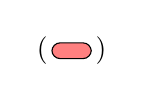
\begin{tikzpicture}[baseline]
                \draw [fill=red!50, rounded corners=3pt]
                    (0, 0) rectangle (0.5, 0.2);
                \node [left=-2pt] at (0, 0.1) {(};
                \node [right=-2pt] at (0.5, 0.1) {)};
            \end{tikzpicture}
            \quad \approx \quad
            \frac 1 \pi  \int \from{-\infty} \till \infty \D \epsilon \,
            \frac \omega {\omega^2 + \epsilon^2}
            \quad
            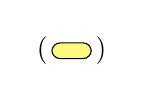
\begin{tikzpicture}[baseline]
                \draw [fill=yellow!50, rounded corners=3pt]
                    (0, 0) rectangle (0.5, 0.2);
                \node [left=-2pt] at (0, 0.1) {(};
                \node [right=-2pt] at (0.5, 0.1) {)};
            \end{tikzpicture}.
        \end{align*}
        %
        The exact integral bears a close resemblance to those which occur in the
        local self energy (Eq.~\ref{local self-energy}).
        }
    \label{constant-DOS approximation}
\end{figure}
%
Save for the factor $N(\epsilon)$, which is unspecified at this point, the
integrands in Eq.~\ref{local self-energy} converge towards zero as $\epsilon$
diverges from $\mu - \chi(\I \omega_m) \approx \mu_0$. Therefore it may be
acceptable to approximate $N(\epsilon)$ by a constant $N(\mu_0)$ \cites [below
Eq.~26]{Allen76} [17]{AllenMitrovic82} [Sec.~B]{MargineGiustino13}, which is
visualized in Fig.~\ref{constant-DOS approximation}, so that the integration can
be performed analytically. With the help of
%
\begin{equation} \label{integrals}
    \frac 1 \pi \int \from{-\infty} \till \infty \D x \frac z {x^2 + z^2}
    = \sgn \Re z
    \quad \text{and} \quad
    \int \from{-\infty} \till \infty \D x \frac x {x^2 + z^2} = 0,
\end{equation}
%
where vanishing and non-vanishing integrals are understood as \textsc{Cauchy}
principal values or follow from the residue theorem, respectively, and writing
$\Delta(\I \omega_n) = \phi(\I \omega_n) / Z(\I \omega_n)$, this yields
%
\begin{equation*}
    \vec \Sigma(\I \omega_n)
    = \pi T \sum_m \frac{ \{
        - \I \omega_m \vec \sigma_0 + \Delta(\I \omega_m) \vec \sigma_1
        \} \lambda(n - m)
        - \Delta(\I \omega_m) \vec \sigma_1 \mu \sub C }
        { \sqrt{\omega_m^2 + \Delta^2(\I \omega_m)} }
\end{equation*}
%
and thus the \emph{cDOS \name{Eliashberg} equations} for a constant density of
states
%
\begin{subequations} \label{cDOS Eliashberg equations}
    \begin{align}
        Z(\I \omega_n) &= 1 + \frac{\pi T}{\omega_n} \sum_m
        \frac{\omega_m}{\sqrt{\omega_m^2 + \Delta^2(\I \omega_m)}}
        \lambda(n - m),
        \\
        \Delta(\I \omega_n) &= \frac{\pi T}{Z(\I \omega_n)} \sum_m
        \frac{\Delta(\I \omega_m)}{\sqrt{\omega_m^2 + \Delta^2(\I \omega_m)}}
        [\lambda(n - m) - \mu \sub C].
    \end{align}
\end{subequations}
%
The chemical potential and the energy shift have disappeared from the equations
and the density of states enters through the coupling strengths only.

\section{Real-axis equations}

In this section the analytic continuation of the self-energy or the
corresponding \name{Eliashberg} equations, which is complicated by the summation
over \name{Matsubara} frequencies, is performed within the constant-DOS
approximation.

The first step is to withdraw the dependence on \name{Matsubara} frequencies
from the \name{Green} function using a spectral representation. Undoing the
energy integration and applying Eq.~\ref{spectral representation},
%
\begin{equation*}
    \int \from{-\infty} \till \infty \D \epsilon \, \vec G_\epsilon(\I \omega_n)
    = -\frac 1 \pi
    \int \from{-\infty} \till \infty \D \omega' \,
    \frac 1 {\I \omega_n - \omega'}
    \Im \int \from{-\infty} \till \infty \D \epsilon \,
    \vec G_\epsilon(\omega'_+),
\end{equation*}
%
where $\omega'_+ = \omega' + \I 0^+$. The \name{Green} function matrix,
analytically continued to arbitrary frequency arguments $\omega$ and dependent
on energy $\epsilon_{\vec k}$ rather than wave number $\vec k$, reads
%
\begin{equation*}
    \vec G_\epsilon(\omega) = \frac
        { \omega Z(\omega) \vec \sigma_0
        + \phi(\omega) \vec \sigma_1
        + \epsilon \vec \sigma_3 }
        { \omega^2 Z^2(\omega)
        - \phi^2(\omega)
        - \epsilon^2}.
\end{equation*}
%
Using Eqs.~\ref{integrals} one finds, in accordance with Eq.~2.19a of
Ref.~\barecite{ScalapinoSchriefferWilkins66},
%
\begin{equation*}
    -\frac 1 \pi \int \from{-\infty} \till \infty \D \epsilon \,
    \vec G_\epsilon(\omega)
    = \frac
        {\omega Z(\omega) \vec \sigma_0 + \phi(\omega) \vec \sigma_1}
        {\sqrt{-\omega^2 Z^2(\omega) + \phi^2(\omega)}}
    = \I \frac
        {\omega Z(\omega) \vec \sigma_0 + \phi(\omega) \vec \sigma_1}
        {\sqrt[\dagger]{\omega^2 Z^2(\omega) - \phi^2(\omega)}}
    = \I \frac
        {\omega \vec \sigma_0 + \Delta(\omega) \vec \sigma_1}
        {\sqrt[*]{\omega^2 - \Delta^2(\omega)}}.
\end{equation*}
%
For the integral to be correct, the first square must have a positive real part.
Since a multiplication with $\I$ corresponds to a rotation by $\frac \pi 2$ in
the complex plane, the second square root must be taken from the upper
half-plane \cite[Eq.~2.19b]{ScalapinoSchriefferWilkins66}. Accordingly the
domain of the third square root is the upper half-plane rotated clockwise by the
complex argument of $Z(\omega)$.

Using $\Im[\I \dots] = \Re[\,\dots]$, the phononic part of the self-energy reads
%
\begin{multline*}
    \vec \Sigma \super{ph.} (\I \omega_n)
    = T \sum_m \int \from{-\infty} \till \infty \D \epsilon \,
    \vec \sigma_3 \, \vec G_\epsilon(\I \omega_m) \, \vec \sigma_3 \,
    \lambda(n - m)
    \\
    = T \int \from{-\infty} \till \infty \D \omega' \, \Re \bigg[ \frac
        {\omega'_+ \vec \sigma_0 - \Delta(\omega'_+) \vec \sigma_1}
        {\sqrt[*]{\omega'^2_+ - \Delta^2(\omega'_+)}}
    \bigg]
    \int \from 0 \till \infty \D \omega'' \, \alpha^2 F(\omega'')
    \sum_m \frac 1 {\I \omega_m - \omega'}
    \frac{2 \omega''}{(\omega_n - \omega_m)^2 + \omega''^2}.
\end{multline*}
%
It is now possible to eliminate the summation over \name{Matsubara} frequencies
\cite[Eqs.~3.40, 3.41]{AllenMitrovic82},
%
\begin{equation*}
    T \sum_m \frac 1 {\I \omega_m - \omega'}
    \frac{2 \omega''}{(\omega_n - \omega_m)^2 + \omega''^2}
    = \frac{f_+(-\omega') + f_-(\omega'')}{\I \omega_n - \omega' - \omega''}
    + \frac{f_+( \omega') + f_-(\omega'')}{\I \omega_n - \omega' + \omega''}
    \equiv \Omega(\I \omega_n, \omega', \omega''),
\end{equation*}
%
and to analytically continue the self-energy, which yields
%
\begin{equation*}
    \vec \Sigma \super{ph.} (\omega) =
    \int \from{-\infty} \till \infty \D \omega' \,
    \Re \bigg[ \frac
        {\omega'_+ \vec \sigma_0 - \Delta(\omega'_+) \vec \sigma_1}
        {\sqrt[*]{\omega'^2_+ - \Delta^2(\omega'_+)}}
    \bigg]
    \int \from 0 \till \infty \D \omega'' \, \alpha^2 F(\omega'') \,
    \Omega(\omega, \omega', \omega'').
\end{equation*}

With the identity \cite[Eq.~12.4]{AllenMitrovic82}
%
\begin{equation} \label{Matsubara sum}
    T \sum_m \frac 1 {\I \omega_m - \omega'} = -\frac 1 2 [1 - 2 f_+(\omega')]
\end{equation}
%
the electronic part of the self-energy is analogously found to be
%
\begin{align*}
    \vec \Sigma \super{el.} (\omega)
    = \mu \sub C T \sum_{m} \int \from{-\infty} \till \infty \D \epsilon \,
    \vec G_{\vec q} \super{od.} (\omega)
    = -\frac {\mu \sub C} 2 \int \from{-\infty} \till \infty \D \omega' \,
    \Re \bigg[ \frac
        {\Delta(\omega'_+) \vec \sigma_1}
        {\sqrt[*]{\omega'^2_+ - \Delta^2(\omega'_+)}}
    \bigg] [1 - 2 f_+(\omega')].
\end{align*}

Thus for $\vec \Sigma(\omega) = \vec \Sigma \super{ph.}(\omega) + \vec \Sigma
\super{el.}(\omega)$ the so-called \emph{real-axis Eliashberg equations}, which
are actually defined for the whole complex plane, read
%
\begin{align*}
    Z(\omega) = 1 - \frac 1 \omega
    &\int \from{-\infty} \till \infty \D \omega' \,
    \Re \bigg[
        \frac{\omega'_+}{\sqrt[*]{\omega'^2_+ - \Delta^2(\omega'_+)}}
    \bigg] \int \from 0 \till \infty \D \omega'' \, \alpha^2 F(\omega'') \,
    \Omega(\omega, \omega', \omega''),
    \\
    \Delta(\omega) = -\frac 1 {Z(\omega)}
    &\int \from{-\infty} \till \infty \D \omega' \,
    \Re \bigg[
        \frac{\Delta(\omega'_+)}{\sqrt[*]{\omega'^2_+ - \Delta^2(\omega'_+)}}
    \bigg]
    \bigg \{
        [1 - 2 f_+(\omega')] \, \frac {\mu \sub C} 2
        + \int \from 0 \till \infty \D \omega'' \, \alpha^2 F(\omega'') \,
        \Omega(\omega, \omega', \omega'')
    \bigg \}.
\end{align*}

Noting that $\lambda(n) = \lambda(-n)$, one can easily verify that even
functions $Z(\I \omega_n)$ and $\Delta(\I \omega_n)$ are perfectly compatible
with Eqs.~\ref{cDOS Eliashberg equations}. This property is inherited by the
corresponding real-axis quantities. More general: Let $f(\omega)$ represent any
of the functions $\omega^2$, $Z(\omega)$ and $\Delta(\omega)$. They all have in
common that they transform into their complex conjugate if the sign of either
the real or imaginary part of their argument changes
\cite[Eq.~A5]{AmbegaokarTewordt64}. Formally,
%
\begin{equation} \label{frequency symmetries}
    f(-\omega) = f(\omega) \quad \text{and} \quad f(\omega^*) = f^*(\omega).
\end{equation}
%
The same applies to functions which are derived by means of the four basic
arithmetical operations, such as $\omega^2 - \Delta^2(\omega)$. Besides, complex
conjugation of a number reflects its possible square roots across the axes of
the complex plane. As a consequence, if $\omega$ is reflected across the real
axis, the same is true for the $Z(\omega)$-dependent domain of $\sqrt[*] \cdots$
and thus for $\sqrt[*]{\omega^2 - \Delta^2(\omega)}$.

This symmetry is now used to fold the negative half of the range of the
$\omega'$ integral onto the positive one, which yields the final form of the
real-axis \name{Eliashberg} equations:
%
\begin{subequations} \label{real-axis Eliashberg equations}
    \begin{align} \notag
        Z(\omega) = 1 - \frac 1 \omega
        &\int \from 0 \till \infty \D \omega' \,
        \Re \bigg[
            \frac{\omega'_+}{\sqrt[*]{\omega'^2_+ - \Delta^2(\omega'_+)}}
        \bigg]
        \times \dots
        \\ \label{Z(omega)}
        \dots \times
        &\int \from 0 \till \infty \D \omega'' \, \alpha^2 F(\omega'') \,
        [ \Omega(\omega,  \omega', \omega'')
        + \Omega(\omega, -\omega', \omega'') ],
        \\ \notag
        \Delta(\omega) = -\frac 1 {Z(\omega)}
        &\int \from 0 \till \infty \D \omega' \,
        \Re \bigg[ \frac
            {\Delta(\omega'_+)}
            {\sqrt[*]{\omega'^2_+ - \Delta^2(\omega'_+)}}
        \bigg]
        \bigg \{
            [1 - 2 f_+(\omega')] \, \mu \sub C
            + \dots
            \\
            \dots +
            &\int \from 0 \till \infty \D \omega'' \, \alpha^2 F(\omega'') \,
            [ \Omega(\omega,  \omega', \omega'')
            - \Omega(\omega, -\omega', \omega'') ]
        \bigg \}.
    \end{align}
\end{subequations}
%
The $\omega$ in the denominator of Eq.~\ref{Z(omega)} is cancelled since, where
braces enclose alternatives,
%
\begin{align*}
    \Omega    (\omega,  \omega', \omega'') \pm
    \Omega    (\omega, -\omega', \omega'') &=
    \Omega_\pm(\omega,  \omega', \omega'') \pm
    \Omega_\pm(\omega, -\omega', \omega''),
    \\
    \Omega_\pm(\omega,  \omega', \omega'') &=
    2 \begin{Bmatrix} \omega \\ \omega' + \omega'' \end{Bmatrix}
    \frac{f_+(-\omega') + f_-(\omega'')}{\omega^2 -(\omega' + \omega'')^2}.
\end{align*}

\section{\name{McMillan}'s formula}

In 1968, William L. \name{McMillan} established a formula to estimate the
transition temperature $T \sub c$ of the superconducting state from only three
characteristic parameters: an average phonon frequency $\av \omega$, the
electron-phonon coupling strength $\lambda$ and the \name{Coulomb}
pseudo-potential $\mu^*$. This section provides a review of the original work
\cite{McMillan68}.

The starting point is a linearized form of the real-axis \name{Eliashberg}
equations, which emerges at $T \sub c$ where $\Delta(\omega)$ is infinitesimal
and negligible relative to $\omega$. Introducing two cutoff energies, the
maximum phonon frequency $\omega_0$ and the electronic bandwidth $E \sub B$, and
assuming that $Z(\omega'_+)$ lies in the upper half-plane or on the positive
real axis so that $\smash{\sqrt[\ast]{\omega'^2_+}} = \omega'_+$,
Eq.~\ref{real-axis Eliashberg equations} becomes
%
\begin{align*}
    Z(\omega) = 1 - \frac 1 \omega
    \int \from 0 \till \infty \D \omega'
    &\int \from 0 \till{\omega_0} \D \omega'' \, \alpha^2 F(\omega'') \,
    [\Omega(\omega, \omega', \omega'') + \Omega(\omega, -\omega', \omega'')],
    \\
    \Delta(\omega) = -\frac 1 {Z(\omega)}
    \int \from 0 \till \infty \D \omega' \,
    \!&\,\frac{\Re[\Delta(\omega')]}{\omega'}
    \Big \{
        \Theta(E \sub B - \omega') \, [1 - 2 f_+(\omega')] \, \mu \sub C
        + \dots
        \\
        \dots +
        &\int \from 0 \till{\omega_0} \D \omega'' \, \alpha^2 F(\omega'') \,
        [\Omega(\omega, \omega', \omega'') - \Omega(\omega, -\omega', \omega'')]
    \Big \}.
\end{align*}

The idea is to find an analytical expression which roughly approximates $T \sub
c$ and can be used to fit numerical results. To that end, a simple trial
function for $\Delta(\omega)$ is introduced, which shall solve the
\name{Eliashberg} equations, i.e. be self-consistent, at least at low and high
frequencies:
%
\begin{equation*}
    \Delta(\omega) = \begin{cases}
        \Delta_0 & \text{for $|\omega| < \omega_0$,} \\
        \Delta_\infty & \text{otherwise,}
    \end{cases}
\end{equation*}
%
where $\Delta_0, \Delta_\infty \in \mathds R$. Several approximate contributions
to $\Delta(0)$ and $\Delta(\infty)$ are taken into account.
%
\begin{enumerate}
    \item \textbf{Phononic contribution to \bm$\Delta(0)$ for \bm$\omega' <
    \omega_0$.} Neglecting $\omega'$ relative to $\omega''$ yields
    %
    \begin{gather*}
        \Omega(0, \omega', \omega'') - \Omega(0, -\omega', \omega'')
        \approx -\frac 2 {\omega''} [1 - 2 f_+(\omega')],
        \\
        \Delta^{(1)}(0) \approx \frac{\Delta_0}{Z(0)}
        \hypo
            {\int_0^{\omega_0} \frac{\D \omega'}{\omega'} [1 - 2 f_+(\omega')]}
            {\approx \ln(\omega_0 / T \sub c)} \
        \hypo
            {2 \int_0^{\omega_0} \frac{\D \omega''}{\omega''}
            \alpha^2 F(\omega'')}{\equiv \lambda},
    \end{gather*}
    %
    where the \emph{electron-phonon coupling strength} $\lambda \equiv
    \lambda(0)$ has reappeared. The integral approximation will be justified in
    Section~\ref{rectangular density of states}, considering that $1 - 2
    f_+(\omega) = \tanh \frac \omega {2 T} \approx \frac 2 \pi \arctan \frac
    \omega T$.
    %
    \item \textbf{Phononic contribution to \bm$\Delta(0)$ for \bm$\omega' \geq
    \omega_0$.} Neglecting $\omega''$ relative to $\omega'$ yields
    %
    \begin{gather*}
        \Omega(0, \omega', \omega'') - \Omega(0, -\omega', \omega'')
        \approx -\frac 2 {\omega'} [1 + 2 f_-(\omega'')],
        \\
        \Delta^{(2)}(0) \approx \frac{\Delta_\infty \lambda}{Z(0)}
        \hypo
            {\int_{\omega_0}^\infty \frac{\D \omega'}{\omega'^2}}
            {= 1 / \omega_0} \
        \hypo
            {\frac 2 \lambda \int \from 0 \till{\omega_0} \D \omega'' \,
            \alpha^2 F(\omega'')}{\equiv \av \omega}
        \hypo{[1 + 2 f_-(\omega'')]}{\approx 1},
    \end{gather*}
    %
    where an \emph{average phonon frequency} $\av \omega$ has been defined.
    %
    \item \textbf{Phononic contribution to \bm$\Delta(\infty)$.} This part
    vanishes for $\Omega(\infty, \omega', \omega'') - \Omega(\infty, -\omega',
    \omega'') = 0$.
    %
    \item \textbf{Electronic contribution to \bm$\Delta(0)$.} With the same
    approximations as in $\Delta^{(1)}(0)$ and $\Delta^{(2)}(0)$,
    %
    \begin{equation*}
        \Delta^{(3)}(0) = -\frac{\mu \sub C}{Z(0)} \bigg[
            \Delta_0 \hypo
                { \int_0^{\omega_0} \frac{\D \omega'}{\omega'}
                [1 - 2 f_+(\omega')] }
                {\approx \ln(\omega_0 / T \sub c)}
            + \Delta_\infty \hypo
                {\int_{\omega_0}^{E \sub B}
                \frac{\D \omega'}{\omega'}}{= \ln(E \sub B / \omega_0)}
            \hypo{[1 - 2 f_+(\omega')]}{\approx 1}
        \bigg].
    \end{equation*}
    %
    \item \textbf{Electronic contribution to \bm$\Delta(\infty)$.} Analogous to
    the calculation of $\Delta^{(3)}(0)$,
    %
    \begin{equation*}
        \Delta(\infty) \approx -\frac{\mu \sub C}{Z(\infty)} \bigg[
            \Delta_0 \ln \frac{\omega_0}{T \sub c}
            + \Delta_\infty \ln \frac{E \sub B}{\omega_0}
        \bigg].
    \end{equation*}
\end{enumerate}

The renormalization at low frequencies is assumed to be $Z(0) = Z(\I \omega_0) =
1 + \lambda$, a result which will be derived in Eq.~\ref{normal-state
renormalization}, whereas for high frequencies one trivially has $Z(\infty) =
1$. It is further required that $\Delta(0) \equiv \Delta_0$ and $\Delta(\infty)
\equiv \Delta_\infty$. The latter equation may be solved for $\Delta_\infty$,
which yields
%
\begin{equation} \label{McMillan's Coulomb pseudo-potential}
    \Delta_\infty = -\mu^* \Delta_0 \ln \frac{\omega_0}{T \sub c}
    \quad \text{with} \quad
    \frac 1 {\mu^*} = \frac 1 {\mu \sub C} + \ln \frac{E \sub B}{\omega_0},
\end{equation}
%
where the \emph{\name{Coulomb} pseudo-potential} $\mu^*$ has been defined.
Hence,
%
\begin{equation*}
    \Delta_0 = \Delta^{(1)}(0) + \Delta^{(2)}(0) + \Delta^{(3)}(0)
    = \frac{\Delta_0}{1 + \lambda}
    [\lambda - \lambda \mu^* \av \omega / \omega_0 - \mu^*]
    \ln \frac{\omega_0}{T \sub c}.
\end{equation*}
%
This equation can be solved for $T \sub c$. The resulting formula is then
generalized by the introduction of three fit parameters $A$, $B$ and $C$, in the
course of which the the maximum frequency $\omega_0$ is replaced by the
\name{Debye} frequency $\Theta$:
%
\begin{equation*}
    T \sub c = \omega_0 \exp \bigg[ {-\frac
        {1 + \lambda}
        {\lambda - \lambda \mu^* \av \omega / \omega_0 - \mu^*}}
    \bigg]
    \rightarrow \frac \Theta A \exp \bigg[ {-\frac
        {B \, (1 + \lambda)}
        {\lambda - C \lambda \mu^* - \mu^*}}
    \bigg].
\end{equation*}

For several fixed $T \sub c$ and $\mu^*$ the linearized Eliashberg equations are
now solved for $\lambda$. Thereby, $F(\omega'')$ is chosen to be the phonon
density of states of niobium \cite{NakagawaWoods63} cut off below
$100\,\mathrm{K}$ and $\alpha^2$, which then determines $\lambda$, adjusted to
obtain self-consistency.

These results are used to determine $A$, $B$ and in a second step $C$ via linear
regression:
%
\begin{equation} \label{linear regression formulas}
    \ln \frac \Theta {T \sub c} \overset{\mu^* = 0}
    = \ln A + B \frac{1 + \lambda}{\lambda},
    \quad
    \frac 1 {\mu^*} \bigg[
        \lambda + \frac{B \, (1 + \lambda)}{\ln (A T \sub c / \Theta)}
    \bigg] = 1 + C \lambda.
\end{equation}
%
The values found by \name{McMillan} read $A = 1.45$, $B = 1.04$ and $C = 0.62$.
He also states that for niobium $\Theta = 277\,\unit K$ and $\av \omega =
230\,\unit K$, which allows the alternative pre-factor $\av \omega / 1.20$ in
place of $\Theta / 1.45$, which should be preferred according to \name{Dynes}
\cite{Dynes72} for a more universal validity.

\section{\name{Coulomb} pseudo-potential}

The introduction of the \name{Coulomb} pseudo-potential in the preceding section
requires a more detailed analysis of the \name{Coulomb} interaction as occurring
in the \name{Eliashberg} theory. Before that, however, it is convenient to put
the local and cDOS \name{Eliashberg} equations (Eqs.~\ref{local Eliashberg
equations} and \ref{cDOS Eliashberg equations}) into a form which is more
suitable for both further analysis and computational implementation.

As already stated in Eq.~\ref{frequency symmetries}, one can assume the
solutions of the Eliashberg equations to be even function of frequency.
Exploiting this symmetry it is possible to fold the negative half of the
\name{Matsubara} sum onto the positive one. For local self-energies this yields
%
\begin{align*}
    Z(\I \omega_n) &= 1 + \frac T {\omega_n} \sum_{m = 0}^\infty
    \int \from{-\infty} \till \infty \D \epsilon
    \frac{N(\epsilon)}{N(\mu_0)}
    \frac{\omega_m Z(\I \omega_m)}{\Theta(\epsilon, m)}
    \Lambda^-(n, m),
    \\
    \phi(\I \omega_n) &= T \sum_{m = 0}^\infty
    \int \from{-\infty} \till \infty \D \epsilon
    \frac{N(\epsilon)}{N(\mu_0)}
    \frac{\phi(\I \omega_m)}{\Theta(\epsilon, m)}
    [\Lambda^+(n, m) - 2 \mu \sub C],
    \\
    \chi(\I \omega_n) &= -T \sum_{m = 0}^\infty
    \int \from{-\infty} \till \infty \D \epsilon
    \frac{N(\epsilon)}{N(\mu_0)}
    \frac{\epsilon - \mu + \chi(\I \omega_m)}{\Theta(\epsilon, m)}
    \Lambda^+(n, m)
\end{align*}
%
and under the additional assumption of a constant density of states
%
\begin{align*}
    Z(\I \omega_n) &= 1 + \frac{\pi T}{\omega_n} \sum_{m = 0}^\infty
    \frac
        {\omega_m Z(\omega_m)}
        {\sqrt{[\omega_m Z(\I \omega_m)]^2 + \phi^2(\I \omega_m)}}
    \Lambda^-(n, m),
    \\
    \phi(\I \omega_n) &= \pi T \sum_{m = 0}^\infty
    \frac
        {\phi(\I \omega_m)}
        {\sqrt{[\omega_m Z(\I \omega_m)]^2 + \phi^2(\I \omega_m)}}
    [\Lambda^+(n, m) - 2 \mu \sub C].
\end{align*}
%
The occurring electron-phonon coupling matrices are defined as
%
\begin{equation*}
    \Lambda^\pm(n, m) = \lambda(n - m) \pm \lambda(n + m + 1).
\end{equation*}

Solving the above equations on a computer requires a truncation of the infinite
summation over \textsc{Matsubara} frequencies. For the phonon part this is
unproblematic since it has a natural cutoff through $\lambda(n)$, which decays
rapidly with growing magnitude of $\nu_n$. The \textsc{Coulomb} part, however,
does not depend on frequency and thus couples terms regardless of the difference
of their frequency arguments. As a consequence, the partial sum does converge
very slowly -- or not at all -- with increasing cutoff. The following procedure%
%
\footnote{Analogous derivations are given by \name{Schrieffer}
\cite[185-188]{Schrieffer83} and \name{Allen} and \name{Mitrovi\'{c}}
\cite[Sec.~9]{AllenMitrovic82}. According to the former, the formula for $\mu^*$
was first given in 1959 by \name{Bogoliubov}, \name{Tolmachev} and
\name{Shirkov} \cite[83]{BogoliubovTolmachevShirkov59}. Nevertheless, the
quantity is named after Pierre \textsc{Morel} and Philip W. \textsc{Anderson}
with reference to Ref.~\barecite{MorelAnderson62} from 1962.}
%
circumvents this.

\subsection{Introduction of frequency cutoff}
\label{introduction of frequency cutoff}

Let $\phi(\I \omega_n) = \phi \sub{ph.} (\I \omega_n) + \phi \sub{el.}$ and
consider the \textsc{Eliashberg} equation for $\phi \sub{el.}$,
%
\begin{equation} \label{constant Coulomb contribution}
    \phi \sub{el.} = -2 \mu \sub C T \sum_{m = 0}^\infty
    \int \from{-\infty} \till \infty \D \epsilon
    \frac{N(\epsilon)}{N(\mu_0)}
    \frac{\phi(\I \omega_m)}{\Theta(\epsilon, m)},
\end{equation}
%
As can be seen from the results presented in Chapter ??, there is a cutoff
frequency $\omega_N$ above which one can safely assume $\phi \sub{ph.} (\I
\omega_m) \approx \chi(\I \omega_m) \approx 0$, $\phi \sub{el.} \ll \omega_m$
and $Z(\I \omega_m) \approx 1$ such that
%
\begin{equation*}
    -2 \mu \sub C T \sum_{m = N}^\infty
    \int \from{-\infty} \till \infty \D \epsilon
    \frac{N(\epsilon)}{N(\mu_0)}
    \frac{\phi(\I \omega_m)}{\Theta(\epsilon, m)}
    \approx -2 \mu \sub C T \sum_{m = N}^\infty
    \int \from{-\infty} \till \infty \D \epsilon
    \frac{N(\epsilon)}{N(\mu_0)}
    \frac{\phi \sub{el.}}{\omega_m^2 + (\epsilon - \mu)^2}.
\end{equation*}
%
Bringing this part to the left-hand side of Eq.~\ref{constant Coulomb
contribution} yields
%
\begin{equation*}
    \bigg[
        1 + 2 \mu \sub C T \sum_{m = N}^\infty
        \int \from{-\infty} \till \infty \D \epsilon
        \frac{N(\epsilon)}{N(\mu_0)}
        \frac 1 {\omega_m^2 + (\epsilon - \mu)^2}
    \bigg]
    \phi \sub{el.} =
    -2 \mu \sub C T \sum_{m = 0}^{N - 1}
    \int \from{-\infty} \till \infty \D \epsilon
    \frac{N(\epsilon)}{N(\mu_0)}
    \frac{\phi(\I \omega_m)}{\Theta(\epsilon, m)}
\end{equation*}
%
or equivalently, introducing a rescaled pseudo-potential $\mu^*(N)$,
%
\begin{equation*}
    \phi \sub{el.} =
    -2 \mu^*(N) T \sum_{m = 0}^{N - 1}
    \int \from{-\infty} \till \infty \D \epsilon
    \frac{N(\epsilon)}{N(\mu_0)}
    \frac{\phi(\I \omega_m)}{\Theta(\epsilon, m)},
    \quad
    \frac 1 {\mu^*(N)} = \frac 1 {\mu \sub C}
    + 2 T \sum_{m = N}^\infty
    \int \from{-\infty} \till \infty \D \epsilon
    \frac{N(\epsilon)}{N(\mu_0)}
    \frac 1 {\omega_m^2 + (\epsilon - \mu)^2}.
\end{equation*}
%
The truncation of the \name{Matsubara} sum has thus been compensated by
rescaling the \name{Couloumb} interaction. For a computational solution for
$\mu^*$ it is further convenient to replace the infinite sum by a closed form.
This is done by means of the identity \cite[Eq.~A.14]{AllenMitrovic82}
%
\begin{equation*}
    \sum_{n = 0}^{N - 1} \frac x {(n + \tfrac 1 2)^2 + x^2}
    = \Im[\psi(\tfrac 1 2 + \I x) - \psi(N + \tfrac 1 2 + \I x)],
\end{equation*}
%
where $\psi(x) = \varGamma'(x) / \varGamma(x)$ is the digamma function which
asymptotically approaches the natural logarithm for large arguments, as found
via the \textsc{Stirling} formula \cite[Appendix~A]{AllenMitrovic82}.
Consequently,
%
\begin{align*}
    \smash[b]{\sum_{n = N}^\infty \frac x {(n + \tfrac 1 2)^2 + x^2}}
    &= \lim_{M \rightarrow \infty}
    \big\{
        \Im[\psi(N + \tfrac 1 2 + \I x) - \psi(M + \tfrac 1 2 + \I x)]
    \big\}
    \\
    &\approx \lim_{M \rightarrow \infty}
    \big\{
        \Im[\log(N + \tfrac 1 2 + \I x) - \log(M + \tfrac 1 2 + \I x)]
    \big\}
    \\
    &= \lim_{M \rightarrow \infty}
    \big\{
        \arg(N + \tfrac 1 2 + \I x)
        - \hypo{\arg(M + \tfrac 1 2 + \I x)}{\rightarrow 0}
    \big\}
    = \smash{\arctan \frac x {N + \tfrac 1 2}}.
\end{align*}
%
and thus, removing the singularity at $\epsilon = \mu$ which not known in
advance and approximated by $\mu_0$ to obtain a formula which can be applied
\emph{before} the \name{Eliashberg} equations are solved,
%
\begin{equation} \label{rescaled Coulomb pseudo-potential}
    \frac 1 {\mu^*(N)} = \frac 1 {\mu \sub C}
    + \frac 1 \pi \int \from{-\infty} \till \infty \D \epsilon
    \frac{N(\epsilon)}{N(\mu_0)}
    \begin{cases}
        \frac 1 {\epsilon - \mu} \arctan \frac{\epsilon - \mu}{\omega_N}
            & \text{for $\epsilon \neq \mu$,} \\
        \frac 1 {\omega_N}
            & \text{otherwise.}
    \end{cases}
\end{equation}

\subsection{Rectangular density of states}
\label{rectangular density of states}

For the special case of a density of states which is constant on the interval
$[-D, D]$ and zero elsewhere and assuming a chemical potential $\mu = 0$
\cite[39]{AllenMitrovic82}, the formula for $\mu^*$ reduces to
%
\begin{equation*}
    \frac 1 {\mu^*(N)} = \frac 1 {\mu \sub C} + R(N)
    \quad \text{with} \quad
    R(N) = \frac 2 \pi \int_0^D \frac {\D \epsilon} \epsilon
    \arctan \frac \epsilon {\omega_N}.
\end{equation*}
%
By means of substitution and partial integration one can further evaluate
%
\begin{equation*}
    R(N) = \frac 2 \pi \int_0^{\frac D {\omega_N}} \frac {\D x} x \arctan x
    = \frac{\arctan \tfrac D {\omega_N}}{\pi / 2} \ln \frac D {\omega_N}
    - \hypo
        {\frac 2 \pi \int_0^{\frac D {\omega_N}} \frac{\D x \, \ln x}{1 + x^2}}
        { \frac 2 \pi \int_{-\infty}^{\ln \frac D {\omega_N}}
        \frac{x \, \D x}{\E^{-x} + \E^x}
        = -\frac 1 \pi \int_{\ln \frac D {\omega_N}}^\infty
        \frac{x \, \D x}{\cosh x} }
\end{equation*}
%
Since the hyperbolic cosine growths exponentially with the magnitude of its
arguments while the arc tangents approaches $\pi / 2$, for the reasonable
assumption $D \gg \omega_N$ one finds
%
\begin{equation} \label{rectangular-DOS mu*}
R(N) = \hyper{\frac{\arctan \tfrac D {\omega_N}}{\pi / 2}}{\approx 1}
\ln \frac D {\omega_N}
+ \hyper{
    \frac 1 \pi \int_{\ln \frac D {\omega_N}}^\infty
    \frac{x \, \D x}{\cosh x}
    }
    {\approx 0}
\quad \text{so that} \quad
\frac 1 {\mu^*(N)} = \frac 1 {\mu \sub C} + \ln \frac D {\omega_N}.
\end{equation}

For the sake of completeness it shall also be mentioned that an exact evaluation
of $R(N)$ is possible in terms of dilogarithms:
%
\begin{equation*}
    R(N) = \frac 1 {\I \pi} \int_0^{\I \frac D {\omega_N}} \frac {\D x} x
    [\ln(1 + x) - \ln(1 - x)]
    \equiv \frac
        { \mathrm{Li}_2 \big(  \I \tfrac D {\omega_N} \big)
        - \mathrm{Li}_2 \big( -\I \tfrac D {\omega_N} \big) }
        {\I \pi}.
\end{equation*}

\subsection{Constant density of states}

One ought to think that the latest results should be directly applicable to the
case of a constant density of states which extends over the whole energy domain.
The problem is, however, that within the approximations made $\mu^*$ would
vanish as $D \rightarrow \infty$, regardless of the chosen cutoff.

A well-defined rescaling prescription can be found by applying the steps carried
out in Section~\ref{introduction of frequency cutoff} directly to the
approximate \name{Eliashberg} equation
%
\begin{equation} \label{approximate constant Coulomb contribution}
    \phi \sub{el.} = -2 \mu^*(M) \pi T \sum_{m = 0}^{N - 1}
    \frac
        {\phi(\I \omega_m)}
        {\sqrt{[\omega_m Z(\I \omega_m)]^2 + \phi^2(\I \omega_m)}},
\end{equation}
%
where an upper cutoff at $\omega_M$ has been introduced in the first place and
the appropriate yet unknown $\mu^*(M)$ is used. The idea is to truncate the
Coulomb part at a lower frequency $\omega_N$, above which $\phi \sub{ph.} (\I
\omega_m) \approx 0$, $\phi \sub{el.} \ll \omega_m$ and $Z(\I \omega_m) \approx
1$ is still a valid assumption. One has
%
\begin{equation*}
    -2 \mu^*(M) \pi T \sum_{m = N}^{M - 1}
    \frac
        {\phi(\I \omega_m)}
        {\sqrt{[\omega_m Z(\I \omega_m)]^2 + \phi^2(\I \omega_m)}}
    \approx -2 \mu^*(M) \pi T \sum_{m = N}^{M - 1}
    \frac{\phi \sub{el.}}{\omega_m}
\end{equation*}
%
which leads to
%
\begin{equation*}
    \phi \sub{el.} = -2 \mu^*(N) \pi T \sum_{m = 0}^{N - 1}
    \frac
        {\phi(\I \omega_m)}
        {\sqrt{[\omega_m Z(\I \omega_m)]^2 + \phi^2(\I \omega_m)}},
    \quad
    \mu^*(N) = \frac{\mu^*(M)}{1 + 2 \mu^*(M) \pi T
    \sum_{m = N}^{M - 1} \omega_m^{-1}},
\end{equation*}
%
As above, one can further simplify
%
\begin{equation*}
    2 \pi T \sum_{m = N}^{M - 1} |\omega_m|^{-1}
    = \sum_{m = N}^{M - 1} \frac 1 {m + \frac 1 2}
    = \psi(M + \tfrac 1 2) - \psi(N + \tfrac 1 2)
    \approx \log \frac{N + \frac 1 2}{N + \frac 1 2}
    = \ln \frac{\omega_M}{\omega_N},
\end{equation*}
%
where Eq.~A.7 of Ref.~\barecite{AllenMitrovic82} has been used. Hence,
%
\begin{equation*}
    \frac 1 {\mu^*(N)} = \frac 1 {\mu^*(M)} + \ln \frac{\omega_M}{\omega_N}.
\end{equation*}
%
From comparison with Eq.~\ref{rectangular-DOS mu*} it follows that the cDOS
approach reproduces the expected results if the non-rescaled $\mu \sub C$ is
used in combination with a cutoff frequency equal to the virtual band-width $D$.
The cDOS approximation thus \emph{requires} a frequency cutoff.

Since $D$ is theoretically infinite and practically unknown it is eliminated by
the assumption that it be equal to the band-width from the derivation of
\name{McMillan's} equation. Combination of the results from Eqs.~\ref{McMillan's
Coulomb pseudo-potential} and \ref{rectangular-DOS mu*} yields the formula to be
used within the imaginary-axis cDOS \name{Eliashberg} equations
\cite[Eq.~13]{AllenDynes75}:
%
\begin{equation} \label{cDOS rescaled Coulomb pseudo-potential}
    \frac 1 {\mu^*(N)} = \frac 1 {\mu^*} + \ln \frac{\omega_0}{\omega_N}.
\end{equation}

\section{Chemical potential}
\label{chemical potential}

If the chemical potential in the \name{Eliashberg} equations is assumed to be
constant, the particle number is not necessarily conserved. Following
Ref.~\barecite{SchafrothRodriguezNunezBeck97}, with the help of
\name{Dirichlet}'s theorem for \name{Fourier} series and
Eq.~\ref{Matsubara-Green function} one finds
%
\begin{align*}
    \av{\op c_{\vec k}^+ \, \op c_{\vec k}}
    = 1 - \av{\op c_{\vec k} \, \op c_{\vec k}^+}
    &= \frac { 1
        + \av{\op c_{\vec k}^+ \, \op c_{\vec k}}
        - \av{\op c_{\vec k} \, \op c_{\vec k}^+}
        } 2
    \\
    &= \frac {1 + G_{\vec k}(0^-) + G_{\vec k}(0^+)} 2
    = \frac 1 2 + G_{\vec k}(0)
    = \frac 1 2 + \frac 1 \beta \sum_{n \in \mathds Z} G_{\vec k}(\I \omega_n)
\end{align*}
%
and thus the \emph{particle density} or \emph{occupation number} per unit cell
%
\begin{equation*}
    n = \frac 1 N \sum_{\vec k \sigma} \av{\op c_{\vec k}^+ \, \op c_{\vec k}}
    = 1 + \frac 2 {\beta N} \sum_{\vec k n} G_{\vec k}(\I \omega_n)
    = 1 - \frac 2 {\beta N} \sum_{\vec k n} \frac
        {\epsilon_{\vec k} - \mu + \chi_{\vec k}(\I \omega_n)}
        {\Theta_{\vec k}(n)},
\end{equation*}
%
where terms with $\I \omega_n Z_{\vec k}(\I \omega_n)$ have cancelled.

\subsection{Free particles}

Using Eq.~\ref{Matsubara sum} it can be shown that for $Z_{\vec k}(\I \omega_n)
= 1$ and $\phi_{\vec k}(\I \omega_n) = \chi_{\vec k}(\I \omega_n) = 0$ the
free-particle occupation number is reproduced:
%
\begin{multline*}
    n = 1 - \frac 2 {\beta N} \sum_{\vec k n}
    \frac
        {\textcolor{gray}{\I \omega_n + {}} \epsilon_{\vec k} - \mu}
        {\omega_n^2 + (\epsilon_{\vec k} - \mu)^2}
    = 1 - \frac 2 {\beta N} \sum_{\vec k n}
    \frac 1 {\epsilon_{\vec k} - \mu - \I \omega_n}
    = \frac 2 N \sum_k f_+(\epsilon_k)
    \\
    = 2 \int \from{-\infty} \till \infty \D \epsilon \,
    n(\epsilon) \, f_+(\epsilon)
    = 1 - \int \from{-\infty} \till \infty \D \epsilon \,
    n(\epsilon) \tanh \frac{\epsilon - \mu}{2 T}.
\end{multline*}
%
This equation could be solved for $\mu$ using a bisection method or the
fixed-point equation
%
\begin{equation*}
    \mu = \frac
        {n - 1 + \int_{-\infty}^\infty \D \epsilon \, \epsilon \, w(\epsilon)}
        {\int_{-\infty}^\infty \D \epsilon \, w(\epsilon)}
    \quad \text{with} \quad
    w(\epsilon) = n(\epsilon)
    \begin{cases}
       \frac 1 {\epsilon - \mu} \tanh \frac{\epsilon - \mu}{2 T}
          & \text{for $\epsilon \neq \mu$,} \\
       \frac 1 {2 T}
          & \text{otherwise.}
    \end{cases}
\end{equation*}
%
For half-filling, i.e. $n = 1$, this gives simply the \emph{center of mass} of
the weight function $w(\epsilon)$.

\subsection{Interacting particles}

The calculation of the occupation number from the results of the imaginary-axis
\name{Eliashberg} equations is complicated by the cutoff of the \name{Matsubara}
sums. A reasonable approximation consists of replacing the unknown part by the
corresponding free-particle expression:
%
\begin{equation*}
    n \approx 1 - 4 T \int \from{-\infty} \till \infty \D \epsilon \,
    n(\epsilon)
    \Bigg[
        \sum_{n = 0}^{N - 1}
        \frac{\epsilon - \mu + \chi(\I \omega_n)}{\Theta(\epsilon, n)}
        + \hypo { \sum_{n = N}^\infty
            \frac{\epsilon - \mu}{\omega_n^2 + (\epsilon - \mu)^2} }
            {\approx \frac 1 {2 \pi T} \arctan \frac{\epsilon - \mu}{\omega_N}}
    \Bigg].
\end{equation*}
%
where the intermediate results from Section \ref{introduction of frequency
cutoff} have been used. Solving this equation for the left appearance of $\mu$
yields a manageable fixed-point equation, namely
%
\begin{align*}
    \mu &\approx \frac
    {
        \frac{n - 1}{4 T} + \int_{-\infty}^\infty \D \epsilon \, n(\epsilon)
        \big[
            \sum_{n = 0}^{N - 1}
            \frac{\epsilon + \chi(\I \omega_n)}{\Theta(\epsilon, n)}
            + \frac 1 {2 \pi T} \arctan \frac{\epsilon - \mu}{\omega_N}
        \big]
    }
    {
        \int_{-\infty}^\infty \D \epsilon \, n(\epsilon)
        \sum_{n = 0}^{N - 1} \frac 1 {\Theta(\epsilon, n)}
    }.
\end{align*}

A fixed-point iteration $x_{n + 1} = f(x_n)$ converges towards a sole fixed
point $\bar x$ if $|f(x) - \bar x| < |x - \bar x|$ for all intermediate values
$x$. At this point it shall not be resolved if the above equations guarantees
convergence for all possible densities of states, self-energies and starting
points. However, in all cases studied convergence at a sufficient rate has been
observed.

\section{Multi-band equations}
\label{multi-band equations}

At this point the most important aspects of \name{Eliashberg} theory for local
self-energies at arbitrary temperatures have been introduced. A straightforward
generalization of the involved equations is with respect to multiple electronic
bands which will turn out to be equivalent to allowing for \name{Fermi}-pocket
resolved anisotropy.

Since a band index is a quantum number just as the wave number, both can be
treated on the same footing. Thus, in \ref{Eliashberg equations} one simply has
to complement the natural occurrences of the wave numbers $\vec k$ and $\vec q$,
even though they have been averaged out as in the case of the \name{Coulomb}
interaction, with band indices $i$ and $j$, respectively. In doing so the
self-energy components searched for are defined for each band separately and
scalar coupling strengths become matrices describing intra- and inter-band
interactions. The corresponding local \name{Eliashberg} equations, where the
band-structure only enters through the density of states, read
%
\begin{subequations} \label{local multi-band Eliashberg equations}
    \begin{align}
        Z_i(\I \omega_n) &= 1 + \frac T {\omega_n} \sum_j \sum_{m = 0}^{N - 1}
        \int \from{-\infty} \till \infty \D \epsilon
        \frac{n_j(\epsilon)}{n_j(\mu_0)}
        \frac{\omega_m Z_j(\I \omega_m)}{\Theta_j(\epsilon, m)}
        \Lambda_{i j}^-(n, m),
        \\
        \phi_i(\I \omega_n) &= T \sum_j \sum_{m = 0}^{N - 1}
        \int \from{-\infty} \till \infty \D \epsilon
        \frac{n_j(\epsilon)}{n_j(\mu_0)}
        \frac{\phi_j(\I \omega_m)}{\Theta_j(\epsilon, m)}
        [\Lambda_{i j}^+(n, m) - 2 \mu^*_{i j}(N)],
        \\
        \chi_i(\I \omega_n) &= -T \sum_j \sum_{m = 0}^{N - 1}
        \int \from{-\infty} \till \infty \D \epsilon
        \frac{n_j(\epsilon)}{n_j(\mu_0)}
        \frac{\epsilon - \mu + \chi_j(\I \omega_m)}{\Theta_j(\epsilon, m)}
        \Lambda_{i j}^+(n, m).
    \end{align}
\end{subequations}
%
The common denominator and the electron-phonon coupling matrices are defined as
%
\begin{align*}
    \Theta_i(\epsilon, n) &= [\omega_n Z_i(\I \omega_n)]^2
    + \phi_i^2(\I \omega_n) + [\epsilon - \mu + \chi_i(\I \omega_n)]^2,
    \\
    \Lambda_{i j}^\pm(n, m)
    &= \lambda_{i j}(n - m) \pm \lambda_{i j}(n + m + 1).
\end{align*}
%
$n_j(\epsilon)$ denotes the density of states for the $j$-th band which is also
part of the definition of the electron-phonon coupling parameter $\lambda_{i j}
\equiv \lambda_{i j}(0) = -n_j(\mu_0) \, g_{i j}^2 \, D(0)$. For symmetric
electron-phonon matrix elements $g_{i j} = g_{j i}$ it follows that $\lambda_{i
j} / \lambda_{j i} = n_j(\mu_0) / n_i(\mu_0)$.

Analogously, for constant band densities of states one finds
%
\begin{subequations} \label{cDOS multi-band Eliashberg equations}
    \begin{align}
        Z_i(\I \omega_n)
        &= 1 + \frac{\pi T}{\omega_n} \sum_j \sum_{m = 0}^{N - 1}
        \frac{\omega_m}{\sqrt{\omega_m^2 + \Delta_j^2(\I \omega_m)}}
        \Lambda_{i j}^-(n, m),
        \\
        \Delta_i(\I \omega_n) &= \frac{\pi T}{Z_i(\I \omega_n)}
        \sum_j \sum_{m = 0}^{N - 1}
        \frac
            {\Delta_j(\I \omega_m)}
            {\sqrt{\omega_m^2 + \Delta_j^2(\I \omega_m)}}
        [\Lambda_{i j}^+(n, m) - 2 \mu^*_{i j}(N)].
    \end{align}
\end{subequations}
%
$\mu^*_{i j}(N)$ is assumed to be rescaled appropriately for the respective set
of equations.

\subsection{Alternate interpretation}

In the multi-band case the summations over band indices are already part of the
underlying interaction \name{Hamilton} operators and find their way through the
\name{Feynman-Dyson} perturbation theory into the \name{Eliashberg} equations.
However, it is also possible to yield formally identical equations within the
single-band formalism.

The basic idea of the local approximation is to reduce the dependence on wave
numbers to a mere energy-dependence. Essentially,
%
\begin{equation*}
    \sum_{\vec k} f(\vec k) \approx
    \int \from{-\infty} \till \infty \D \epsilon \,
    \hyper{\sum_{\vec k} \delta(\epsilon - \epsilon_{\vec k})}{N(\epsilon)} \,
    f(\epsilon).
\end{equation*}
%
If the special case where $f(\vec k)$ is a function of $\epsilon_{\vec k}$ only
the above equation becomes exact. Otherwise $f(\epsilon)$ is an appropriate
constant-energy average.

The alternate idea is now to split the domain of the band-structure, for example
the first \name{Brillouin} zone, into subdomains for which separate densities of
states are determined \cite{Entel76} and the corresponding averages taken.
Formally,
%
\begin{equation*}
    \sum_{\vec k} f(\vec k) \approx
    \sum_i \int \from{-\infty} \till \infty \D \epsilon \,
    \hyper
        {\sum_{\vec k \in D_i} \delta(\epsilon - \epsilon_{\vec k})}
        {N_i(\epsilon)} \,
    f_i(\epsilon)
    \quad \text{where} \quad
    \bigcup_i D_i = \text{\name{Brillouin} zone}.
\end{equation*}
%
Thus the new quantum numbers may also indicate subdomains of the reciprocal
space. This procedure may in turn be generalized with respect to further quantum
numbers such as real band indices.

\section{Linearized equations}

At $T \sub c$, where the order parameter $\Delta(\I \omega_m)$ is infinitesimal,
and in the normal state, where it is zero, it can be neglected relative to
$\omega_m$. Analogous to the derivation of the real-axis \name{Eliashberg}
equations (Eqs.~\ref{real-axis Eliashberg equations}) the cDOS multi-band
imaginary-axis \name{Eliashberg} equations (Eqs.~\ref{cDOS multi-band Eliashberg
equations}) assume the following linearized form:
%
\begin{subequations} \label{linearized cDOS multi-band Eliashberg equations}
    \begin{align}
        Z_i(\I \omega_n)
        &= 1 + \frac 1 {2 n + 1} \sum_j \sum_{m = 0}^{N - 1}
        \Lambda_{i j}^-(n, m),
        \\
        \Delta_i(\I \omega_n) &= \frac 1 {Z_i(\I \omega_n)}
        \sum_j \sum_{m = 0}^{N - 1}
        \frac{\Delta_j(\I \omega_m)}{2 m + 1}
        [\Lambda_{i j}^+(n, m) - 2 \mu^*_{i j}(N)].
    \end{align}
\end{subequations}
%
At this point the equation for $Z_i(\I \omega_n)$ is neither coupled to the
equation of $\Delta_i(\I \omega)$ nor must it be solved self-consistently. For
$N \rightarrow \infty$ can further evaluate
%
\begin{equation} \label{normal-state renormalization}
    Z_i(\I \omega_n) = 1 + \frac 1 {2 n + 1} \sum_j \sum_{m = -n}^n
    \lambda_{i j}(m)
    = 1 + \frac 1 {2 n + 1} \sum_j
    \Big[ \lambda_{i j} + 2 \sum_{m = 1}^n \lambda_{i j}(m) \Big].
\end{equation}
%
This yields the matrix equation $\vec \Delta \cdot \vec K = \vec \Delta$,
component-wise written as
%
\begin{equation}
    \begin{split}
        \Delta_i(\I \omega_n) &= \sum_j \sum_{m = 0}^{N - 1}
        K_{i j}(n, m) \, \Delta_j(\I \omega_m),
        \\
        K_{i j}(n, m) &= \frac 1 {2 m + 1} [\Lambda_{i j}^+(n, m)
        - \delta_{i j} \delta_{n m} D_i^N(n) - 2 \mu^*_{i j}(N)],
        \\
        D_i^N(n) &= \sum_j \sum_{m = 0}^{N - 1} \Lambda_{i j}^-(n, m)
        \overset{N = \infty} =
        \sum_j \Big[ \lambda_{i j} + 2 \sum_{m = 1}^n \lambda_{i j}(m) \Big].
    \end{split}
    \label{linearized gap equation}
\end{equation}
%
Since at temperatures greater than, equal to or less than $T \sub c$
multiplication with the \emph{kernel} $\vec K$ ought to or diminish, maintain or
amplify the magnitude of the order parameter $\vec \Delta$, respectively, $T
\sub c$ is defined as the temperature at which the greatest eigenvalue of $\vec
K$ crosses unity \cite[47]{AllenMitrovic82}.

Before the analysis can go more into detail it necessary to introduce the direct
matrix product and its spectral properties, which will be done in the following
section.

\subsection{Direct product}

The \emph{direct product} or \emph{\name{Kronecker} product} $\vec A \otimes
\vec B$ of the $r \times c$ matrix $\vec A$ and the $R \times C$ matrix $\vec B$
is the $r c \times R C$ matrix defined by
%
\begin{equation*}
    (\vec A \otimes \vec B)_{i j, n m} = A_{i n} B_{j m},
\end{equation*}
%
where $i j, n m$ can be interpreted e.g. as $i R + j, n C + m$ if all indices
are zero-based. This definition also holds for column vectors if these are
considered as, say, $N \times 1$ matrices.

With the help of the identity
%
\begin{equation*}
    (\vec A \otimes \vec B) \cdot (\vec C \otimes \vec D)
    = (\vec A \cdot \vec C) \otimes (\vec B \cdot \vec D)
\end{equation*}
%
which is easily proved component-wise,
%
\begin{multline*}
    [(\vec A \otimes \vec B) \cdot (\vec C \otimes \vec D)]_{i j, p q}
    = \sum_{n m}
        (\vec A \otimes \vec B)_{i j, n m} \,
        (\vec C \otimes \vec D)_{n m, p q}
    = \sum_{n m} A_{i n} B_{j m} C_{n p} D_{m q}
    \\
    = \sum_n A_{i n} C_{n p} \sum_m B_{j m} D_{m q}
    = (\vec A \cdot \vec C)_{i p} \, (\vec B \cdot \vec D)_{j q}
    = [(\vec A \cdot \vec C) \otimes (\vec B \cdot \vec D)]_{i j, p q},
\end{multline*}
%
one can show that, if the eigenvalue equations $\vec A \cdot \vec \alpha = a
\vec \alpha$ and $\vec B \cdot \vec \beta = b \vec \beta$ hold,
%
\begin{equation} \label{eigenvalues direct product}
    (\vec A \otimes \vec B) \cdot (\vec \alpha \otimes \vec \beta)
    = (\vec A \cdot \vec \alpha) \otimes (\vec B \cdot \vec \beta)
    = (a \vec \alpha) \otimes (b \vec \beta)
    = a b (\vec \alpha \otimes \vec \beta).
\end{equation}
%
The eigenvectors and -values of the direct product of two matrix are thus the
direct and normal products of the respective eigenvectors and -values of the
individual matrices.

\subsection{Effective coupling constants}
\label{effective coupling constants}

In the following, two approximations are presented which allow to map the
matrices describing multi-band coupling strengths onto scalar values which lead
to similar critical temperatures. It shall be noted that for all non-scalar
couplings there are always innumerable sets of effective scalar parameters which
yield exactly the same critical temperature -- it is just that there are no
simple rules to generate them.

\subsubsection{Non-renormalized energies}
\label{non-renormalized}

Supposing that there is no energy renormalization, i.e. $Z_i(\I \omega_n) = 1$
for all bands and frequencies, which constitutes a very rough approximation, the
kernel reduces to
%
\begin{equation*}
   K_{i j}(n, m) = \frac 1 {2 m + 1} [\Lambda_{i j}^+(n, m) - 2 \mu^*_{i j}(N)],
\end{equation*}
%
Assuming further that the matrices $\vec \lambda$ and $\vec \mu^*(N)$ describing
the intra- and inter-band electron-phonon coupling strengths and rescaled
\name{Coulomb} pseudo-potentials are proportional, i.e. $\lambda_{i j} = c \,
\mu^*_{i j}(N)$ with $c \ge 0$, one finds the quotient $Q(n, m) \equiv K_{i
j}(n, m) / \lambda_{i j}$ to be independent of band indices. For the
corresponding matrices it follows that
%
\begin{equation*}
    \vec K = \vec Q \otimes \vec \lambda.
\end{equation*}
%
Hence, applying Eq.~\ref{eigenvalues direct product}, the largest eigenvalue of
$\vec K$ is the product of the largest eigenvalues of $\vec Q$ and $\vec
\lambda$ (in magnitude). As a consequence, if there exists a single-band system
with positive coupling strengths $\lambda$ and $\mu^*(N)$ which exhibits the
same critical temperature as a multi-band system with coupling matrices $\vec
\lambda$ and $\vec \mu^*(N)$, then the further would be given by the greatest
eigenvalues of the latter if the renormalization were unity. For two bands and
$\mu^*(N) = 0$,
%
\begin{equation*}
    \lambda = \lambda_{11} + \lambda_{22} + \sqrt{
        (\lambda_{1 1} - \lambda_{2 2})^2 + 4 \lambda_{1 2} \lambda_{2 1}
        }.
\end{equation*}

\subsubsection{Cutoff-independent mapping}
\label{cutoff-independent}

Another approach takes the mapping searched for as independent of the cutoff
frequency $\omega_N$. This allows to derive it for the most simple case where
$N = 1$. Consequently, for $n = m = 1$
%
\begin{equation*}
   K_{i j} = 2 \lambda_{i j} - \delta_{i j} \sum_j \lambda_{i j}
   - 2 \mu^*_{i j}(N),
\end{equation*}
%
where $\lambda_{i j}(1) \approx \lambda_{i j}$ has been assumed additionally.
For two bands and $\mu^*_{i j}(N) = 0$,
%
\begin{equation*}
   \vec K = \begin{bmatrix}
      \lambda_{1 1} - \lambda_{1 2} & 2 \lambda_{1 2} \\
      2 \lambda_{2 1} & \lambda_{2 2} - \lambda_{2 1}
   \end{bmatrix}
\end{equation*}
%
the greatest eigenvalue of which gives the desired approximate effective
couplings strength:
%
\begin{equation*}
   \lambda = \frac 1 2 \bigg[
      \lambda_{1 1} - \lambda_{1 2} - \lambda_{2 1} + \lambda_{2 2}
      + \sqrt{
         (\lambda_{1 1} - \lambda_{1 2} + \lambda_{2 1} - \lambda_{2 2})^2
         + 16 \lambda_{1 2} \lambda_{2 1}
         }
   \bigg].
\end{equation*}

\subsection{Non-constant densities of states}

If the band densities of states are not considered to be constant,
Eqs.~\ref{local multi-band Eliashberg equations} have to be solved. The only
simplification emerging at $T \sub c$ is that the order parameter can be
neglected in the common denominator which becomes $\Theta_i(\epsilon, n) =
[\omega_n Z_i(\I \omega_n)]^2 + [\epsilon - \mu + \chi_i(\I \omega_n)]^2$. As a
consequence, renormalization function and energy shift become decoupled from the
order parameter and may thus be determined independently. Having done so, these
normal-state properties, together with the self-consistent chemical potential,
are inserted into the remaining equation which yields
%
\begin{align*}
    \phi_i(\I \omega_n) &= \sum_j \sum_{m = 0}^{N - 1}
    K_{i j}(n, m) \, \phi_j(\I \omega_m),
    \\
    K_{i j}(n, m) &= T \sub c \int \from{-\infty} \till \infty \D \epsilon
    \frac{n_j(\epsilon)}{n_j(\mu_0)}
    \frac {\Lambda_{i j}^+(n, m) - 2 \mu^*_{i j}(N)}
    {[\omega_m Z_j(\I \omega_m)]^2 + [\epsilon - \mu + \chi_j(\I \omega_m)]^2}.
\end{align*}

\section{\name{Padé} approximants}
\label{Pade approximants}

The imaginary-axis \name{Eliashberg} equations are more convenient for a
computational implementation than the real-axis complements since they involve
sums over already discrete \name{Matsubara} frequencies rather than integrals
the domains of which are yet be be discretized, which is always accompanied by
some loss of accuracy. In addition, no complex quantities are involved.

Since real-axis results can be obtained imaginary-axis results via analytic
continuation (see Eq.~\ref{G(i omega_n)}), being interested in the former it may
still be worth it to take a detour via the latter. Hereby the problem arises,
that an \emph{analytic} continuation can only be applied to some analytic
expression, whereas the numerical results are generally just a finite set of
sample points. In the following a solution proposed by \name{Vidberg} and
\name{Serene} in 1977 \cite{VidbergSerene77} is presented.

Let $\Sigma(\I \omega_n)$ with $n \in \{ 0 \dots N - 1 \}$ act as a placeholder
for any of the self-energy components resulting from the \name{Eliashberg}
equations and derived quantities. The idea is to interpolate this numerical
result by a rational function to which the analytic continuation can then be
applied. This \emph{\name{Padé} approximant} may be written as a continued
fraction
%
\begin{equation} \label{continued fraction}
    \Sigma(\omega) = \dfrac{c_0 \, \phantom{(\omega - \I \omega_0)}}
    {1 + \dfrac{c_1 \, (\omega - \I \omega_0)}
    {1 + \dfrac{c_2 \, (\omega - \I \omega_1)} \dots}}
    \quad \text{with} \quad c_n = 0 \quad \text{for} \quad n \ge N,
\end{equation}
%
where the non-zero coefficients have to be determined so that all imaginary-axis
results are reproduced. For this purpose, \name{Vidberg} and \name{Serene}
propose the following algorithm:
%
\begin{align*}
    & g_0(\I \omega_m)
        \leftarrow \Sigma(\I \omega_m) \quad \text{for all $m$.} \\[4pt]
    & \text{For $n = 0 \dots N - 2$:} \\
    & \qquad g_{n + 1}(\I \omega_m) \leftarrow \frac
        {g_n(\I \omega_n) - g_n(\I \omega_m)}
        {(\I \omega_m - \I \omega_n) g_n(\I \omega_m)}
        \quad \text{for $m > n$.} \\[4pt]
    & c_n \leftarrow g_n(\I \omega_n) \quad \text{for all n.} \\[4pt]
    & \text{For each $\omega \in \mathds R$ of interest:} \\
    & \qquad \vec x_0(\omega) \leftarrow (\rlap 0 \phantom{c_0} \ 1). \\
    & \qquad \vec x_1(\omega) \leftarrow (c_0 \ 1). \\[4pt]
    & \qquad \text{For $n = 1 \dots N - 1$:} \\
    & \qquad \qquad \vec x_{n + 1}(\omega)
        \leftarrow \vec x_n(\omega) + c_n (\omega - \I \omega_{n - 1}) \,
        \vec x_{n - 1}(\omega). \\[4pt]
    & \qquad \Sigma(\omega)
        \leftarrow \frac{[\vec x_N(\omega)]_1}{[\vec x_N(\omega)]_2}. \\
    \intertext{%
        Having determined the coefficients, this algorithm does not calculate
        the continued fraction as stated in Eq.~\ref{continued fraction} but
        rather its representation as a fraction of two polynomials via a
        forward-recurrence formula. This would be favorable if not only the
        final but also intermediate approximants $[\vec x_n(\omega)]_1 / [\vec
        x_n(\omega)]_2$ taking only $n < N$ points into account were needed.
        However, being only interested in the $N$-point \name{Padé} approximant,
        a backward-recurrence algorithm which simply calculates the continued
        fraction successively from \q{tail to head} is preferable for both
        requiring less operations and being numerically more stable
        \cite{JonesThron74}:
        }
    & \text{For each $\omega \in \mathds R$ of interest:} \\
    & \qquad \Sigma(\omega) \leftarrow 1. \\[4pt]
    & \qquad \text{For $n = 1 \dots N - 1$ in reversed order:} \\
    & \qquad \qquad \Sigma(\omega) \leftarrow 1
        + \frac{c_n \, (\omega - \I \omega_{n - 1})}{\Sigma(\omega)}. \\[4pt]
    & \qquad \Sigma(\omega) \leftarrow \frac{c_0}{\Sigma(\omega)}.
\end{align*}
%
The actual implementation for this work can be consulted in
Section~\ref{real_axis}.
